\documentclass[11pt,a4paper]{article}
\usepackage[margin=23mm]{geometry}
\usepackage[T1]{fontenc}
\usepackage{lmodern,microtype}
\usepackage{amsmath,amssymb,bm,mathtools}
\usepackage{siunitx,booktabs,tabularx,longtable,array}
\usepackage{graphicx,tikz,pgfplots}
\usetikzlibrary{arrows.meta,positioning,fit,backgrounds}
\usepgfplotslibrary{groupplots}
\pgfplotsset{compat=1.18}
\usepackage{xurl}
\usepackage[colorlinks=true,linkcolor=blue!55!black,citecolor=blue!55!black,
 urlcolor=blue!55!black,pdftitle={Litter Physics: Formal Model and Implementation},
 pdfauthor={Litter Physics project}]{hyperref}
\usepackage{fancyhdr}
\pagestyle{fancy}
\fancyhf{}
\fancyhead[L]{\small Litter Physics: model and implementation}
\fancyhead[R]{\small Baseline \nolinkurl{9a66a55}}
\fancyfoot[C]{\thepage}
\setlength{\headheight}{14pt}
\setlength{\emergencystretch}{1.5em}
\setlength{\parskip}{.3em}
\numberwithin{equation}{section}
\sisetup{per-mode=symbol,detect-all}
\newcommand{\source}[1]{\href{https://github.com/nredd/litter-physics/blob/9a66a559ed478629d514756662a8fd98a8f52f50/#1}{\nolinkurl{#1}}}
\newcommand{\PelletMassGrams}{0.373221}
\newcommand{\PelletAxialInertia}{1.6795e-09}
\newcommand{\PelletTransverseInertia}{5.3184e-09}
\newcommand{\PelletStepMicroseconds}{61.0918}
\newcommand{\PelletWallOverlapMicrons}{3.66005}
\newcommand{\PelletSubsteps}{17}
\newcommand{\BlockMassGrams}{8}
\newcommand{\BlockPotentialMillijoules}{0.7848}
\newcommand{\HBReturnedStress}{78.006}
\newcommand{\HBPlasticIncrement}{0.00159523}
\newcommand{\HBDissipation}{0.124438}
\newcommand{\HBElasticDrop}{0.126028}
\newcommand{\WaterBulkModulus}{55555.6}
\newcommand{\WaterSoundSpeed}{7.45356}
\newcommand{\WaterBottomPressure}{98.1867}
\newcommand{\WaterBottomRatio}{0.998236}
\newcommand{\WaterAcousticStep}{8.04984e-05}


\title{\textbf{Litter Physics}\\[.4em]
 A formal model, numerical method,\\and implementation audit}
\author{Litter Physics project}
\date{19 September 2026\\[.3em]\small Scientific source baseline: \nolinkurl{9a66a55}}

\begin{document}
\maketitle
\begin{abstract}
This note derives the models currently implemented for a two-box pine-pellet
litter simulation, connects their equations to Rust and Python components, and
separates numerical evidence from intended physical capability. The household
model combines rigid multisphere pellets, frictional contact, timed visit and
maintenance events, and conservative but phenomenological water/fines transport.
Research fixtures use quadratic MLS-MPM with affine particle velocities,
finite-strain viscoplastic paste or weakly compressible liquid, and optional
single-pellet impulse coupling. Worked dimensional examples, constitutive
calculations, method diagrams and archived refinement plots make assumptions
and failure modes explicit. The six-case slump study completes but does not
meet its refinement criterion. Neither full physical energy closure nor
measured household accuracy is established. No calibrated response bridge
between the two numerical scales is yet active.
\end{abstract}

\noindent\textbf{Status of this document.} A source-grounded description of an
executable preliminary model, not a claim that the intended research multiphysics
or an actual household has been validated. The native fidelity labels remain
\nolinkurl{preliminary_household} and \nolinkurl{research_unvalidated}.

\tableofcontents
\clearpage

\section{Problem definition, scope, and two numerical scales}
The physical target is a household using two stainless-steel Sorstrem sifting
boxes filled with pine pellets. Visits disturb and redistribute the bed; liquid
and waste are deposited; wet pellets swell and break down; fines sift into a
drawer; scooping, drawer emptying and topping up alter the next visit's initial
condition. The mathematical target is therefore a persistent state trajectory,
not a collection of independent clean-box scenes:
\begin{equation}
 \mathcal X(t+\Delta t)=\mathcal S_{\Delta t}
     [\mathcal X(t),\boldsymbol\theta,\mathcal E_{[t,t+\Delta t]}],
 \qquad \mathbf y(t)=\mathcal H[\mathcal X(t)].
 \label{eq:state-map}
\end{equation}
$\mathcal X$ contains pellet poses, velocities and contact histories; material
fields and compartments; and cumulative bookkeeping. $\boldsymbol\theta$ denotes
geometry, material and proxy-behavior parameters. $\mathcal E$ is the timed event
sequence; $\mathcal H$ supplies observables. Checkpointing must preserve this
state, not merely a visualization frame.

Two computational scales address different questions. The household scale
retains many discrete pellets and long-lived maintenance state using reduced
material laws. Research fixtures isolate continuum constitutive behavior and
pellet/material interaction at much smaller sizes. The intended eventual
reduction is a measured, verified response $R(\boldsymbol\theta,\mathbf z)$
conditioning household rules on local state $\mathbf z$. That coupling remains
planned, even though a standalone table interpolator already exists.

\begin{figure}[htbp]
\centering
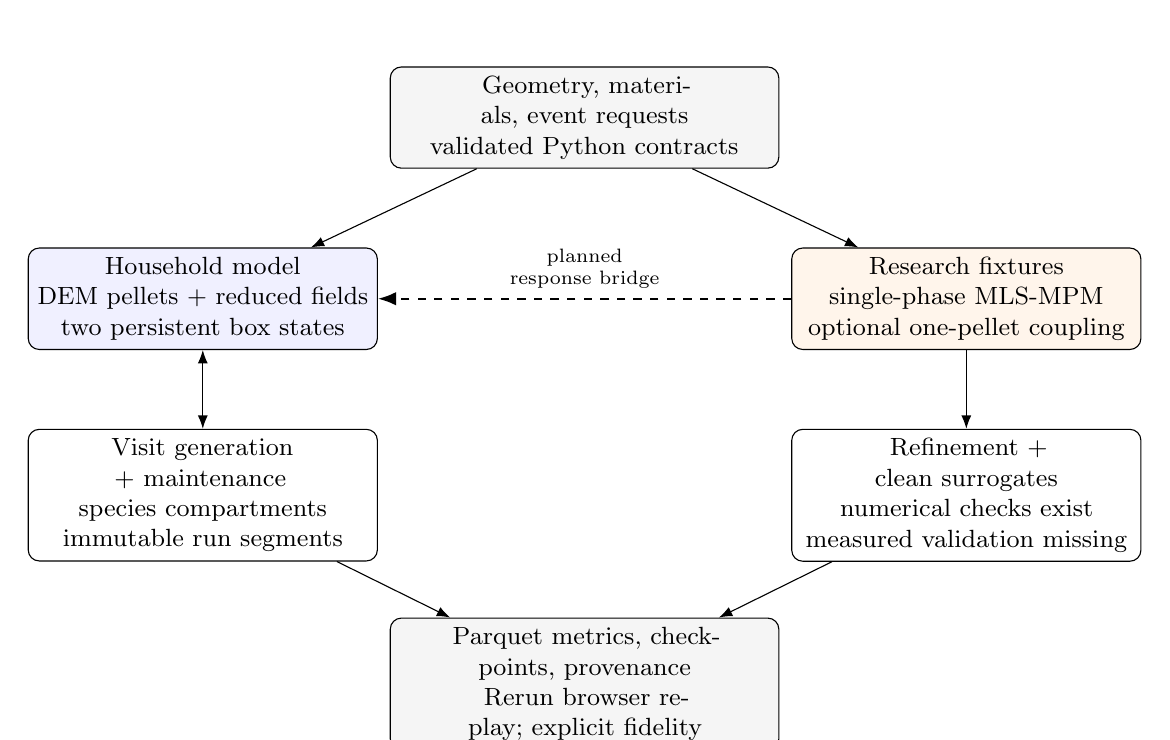
\begin{tikzpicture}[>=Latex,font=\small,
 box/.style={draw,rounded corners,align=center,text width=4.7cm,minimum height=1.15cm},
 smallbox/.style={box,text width=4.2cm}]
 \node[box,fill=gray!8] (input) {Geometry, materials, event requests\\validated Python contracts};
 \node[smallbox,fill=blue!6,below left=1cm and .15cm of input] (house)
 {Household model\\DEM pellets + reduced fields\\two persistent box states};
 \node[smallbox,fill=orange!8,below right=1cm and .15cm of input] (research)
 {Research fixtures\\single-phase MLS-MPM\\optional one-pellet coupling};
 \node[smallbox,below=1cm of house] (events)
 {Visit generation + maintenance\\species compartments\\immutable run segments};
 \node[smallbox,below=1cm of research] (verify)
 {Refinement + clean surrogates\\numerical checks exist\\measured validation missing};
 \node[box,below=5.7cm of input,fill=gray!8] (output)
 {Parquet metrics, checkpoints, provenance\\Rerun browser replay; explicit fidelity};
 \draw[->] (input)--(house); \draw[->] (input)--(research);
 \draw[<->] (house)--(events); \draw[->] (research)--(verify);
 \draw[->] (events)--(output); \draw[->] (verify)--(output);
 \draw[->,dashed,thick] (research.west)--node[above,align=center,font=\scriptsize]
 {planned\\response bridge}(house.east);
\end{tikzpicture}
\caption{Implemented components use solid arrows; the cross-scale response
bridge is not connected. Output and provenance are shared infrastructure, not
proof of equivalent fidelity between the two models.}
\label{fig:architecture}
\end{figure}

\subsection{Evidence and approximation vocabulary}
\begin{description}
 \item[Implemented.] A specific update or diagnostic exists in the pinned source.
 This does not imply accuracy for all inputs.
 \item[Verified in a limited sense.] A stated numerical property has test or run
 evidence, with its fixture, tolerance and scope named.
 \item[Assumed.] A geometry, constant, constitutive closure or behavior distribution
 lacks the measurements needed to identify it for the intended household.
 \item[Planned.] A mathematically motivated extension not executed by this version.
\end{description}
The example dimensions and masses are synthetic. No real cat identities,
per-cat video measurements, pellet distributions or clean-surrogate material
measurements are supplied. A steel-box product name does not determine actual
slot geometry, tolerances, packing fraction, friction or wet behavior.

\subsection{Notation and units}
All solver quantities use SI units; plots sometimes display mm, ms or $\mu$J.
Bold lower-case symbols are vectors, bold upper-case symbols are matrices, and
$A:B=\operatorname{tr}(A^TB)$ is the Frobenius inner product.
$\operatorname{dev}A=A-\tfrac13\operatorname{tr}(A)\mathbf I$.

\begin{center}\small
\begin{tabularx}{\linewidth}{lXl}
\toprule
Symbol & Meaning & Units\\
\midrule
$h,\Delta t$ & Research grid spacing and integration step & m, s\\
$m_p,V_{0p},J$ & Material-point mass, reference volume, volume ratio & kg, m$^3$, 1\\
$\rho_0,\rho$ & Reference and current density & kg/m$^3$\\
$\mathbf C,\mathbf F_e$ & Affine velocity gradient; elastic deformation & s$^{-1}$, 1\\
$\boldsymbol\sigma,\boldsymbol\tau$ & Cauchy and Kirchhoff stresses & Pa\\
$G,K_b,E,\nu_P$ & Shear, bulk, Young's moduli; Poisson ratio & Pa, Pa, Pa, 1\\
$\tau_y,K_s,n$ & Rheometer yield stress, consistency, flow index & Pa, Pa s$^n$, 1\\
$\sigma_y,K_e$ & Equivalent-stress yield and consistency & Pa, Pa s$^n$\\
$\mu,\eta,\nu$ & Contact friction; dynamic and kinematic viscosity & 1, Pa s, m$^2$/s\\
\bottomrule
\end{tabularx}
\end{center}
The household gravity magnitude is \SI{9.80665}{m.s^{-2}}; the research wire
fixtures use \SI{9.81}{m.s^{-2}}. Worked examples below use the corresponding
value. $\nu_P$ is Poisson ratio, distinct from kinematic viscosity $\nu$.

\section{Rigid pellets, contact, and explicit sifting geometry}
\label{sec:dem}
The household kernel is a discrete element model (DEM), in the spirit of
history-dependent granular contact models \cite{cundall}. Its pellets are rigid
multisphere collision proxies, not deformable wood cylinders. A single pellet
has mass $m$, centre $\mathbf{x}$, orientation $\mathbf{R}\in SO(3)$, velocity
$\mathbf{v}$ and angular velocity $\boldsymbol\omega$.

\subsection{Mass properties and multisphere approximation}
For a measured cylinder radius $r$, length $L$, and dry density $\rho_w$, the
assigned mass and body-axis moments are
\begin{equation}
 m=\rho_w\pi r^2L,\qquad I_\parallel=\tfrac12mr^2,\qquad
 I_\perp=\tfrac1{12}m(3r^2+L^2). \label{eq:pellet-inertia}
\end{equation}
These are \emph{cylinder} properties; summing the overlapping collision spheres
would overcount material. Let $a=\max(L-2r,0)$. When $a>0$, set
$n_s=\lceil a/r\rceil+1$ and place sphere centres at
\begin{equation}
 s_k=-\frac a2+\frac{ka}{n_s-1},\qquad
 \mathbf{x}_k=\mathbf{x}+\mathbf{R}\mathbf{e}_\parallel s_k,
 \quad k=0,\ldots,n_s-1. \label{eq:multisphere}
\end{equation}
For $a=0$ there is one sphere. Household pellets allow at most 16 spheres.
The household body axis is $\mathbf{e}_z$; the separate research pellet uses
$\mathbf{e}_x$. Thus their inertia arrays and orientations cannot be copied
between implementations without a basis change.

For a slot along $x$ with width $w$ along $y$, a horizontal pellet at angle
$\theta$ to the slot has collision-envelope width
\begin{equation}
 b_y(\theta)=2r+a|\sin\theta|. \label{eq:slot-envelope}
\end{equation}
The condition $b_y\leq w$ is necessary for this flat orientation to fit between
parallel sides; finite slot length, end bars, vertical tilt and other pellets
also matter. It is not a stochastic ``sift probability.'' With the illustrative
$r=\SI{3}{mm}$ and $w=\SI{5}{mm}$, even $b_y(0)=\SI{6}{mm}>w$:
these \emph{intact} dry pellets cannot pass an ideal slot. Fines are a separate
field representation, not smaller DEM spheres generated by fracture.

\begin{figure}[htbp]
\centering
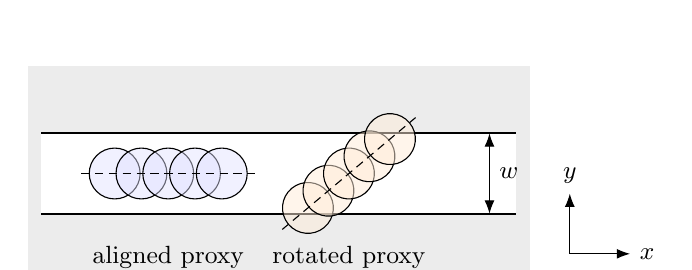
\begin{tikzpicture}[scale=0.85,>=Latex,font=\small]
 \fill[gray!15] (-.5,-1.6) rectangle (7,1.6);
 \fill[white] (-.3,-.6) rectangle (6.8,.6);
 \draw[thick] (-.3,-.6)--(6.8,-.6) (-.3,.6)--(6.8,.6);
 \draw[<->] (6.4,-.6)--node[right]{$w$}(6.4,.6);
 \begin{scope}[shift={(1.6,0)}]
  \foreach \x in {-0.8,-0.4,0,0.4,0.8}{\draw[fill=blue!12,fill opacity=.45] (\x,0) circle (.38);}
  \draw[densely dashed] (-1.3,0)--(1.3,0);
 \end{scope}
 \begin{scope}[shift={(4.3,0)},rotate=40]
  \foreach \x in {-0.8,-0.4,0,0.4,0.8}{\draw[fill=orange!15,fill opacity=.5] (\x,0) circle (.38);}
  \draw[densely dashed] (-1.3,0)--(1.3,0);
 \end{scope}
 \node at (1.6,-1.25) {aligned proxy};
 \node at (4.3,-1.25) {rotated proxy};
 \draw[->] (7.6,-1.2)--(8.5,-1.2) node[right]{$x$};
 \draw[->] (7.6,-1.2)--(7.6,-.3) node[above]{$y$};
\end{tikzpicture}
\caption{Top-view collision schematic, not measured Sorstrem geometry. Sphere
unions set contact geometry while cylinder formulas set mass and inertia.
Rotating the same proxy changes its projected width. The drawing uses a slot
wider than the pellet diameter for illustration, unlike the synthetic example's
\SI{5}{mm} slot.}
\label{fig:slot}
\end{figure}

\subsection{Contact law and history}
Take $\mathbf{n}$ from the second contact partner toward the first. At contact
point $\mathbf{x}_c$, the rigid velocity is
$\mathbf{u}=\mathbf{v}+\boldsymbol\omega\times(\mathbf{x}_c-\mathbf{x})$.
For overlap $\delta>0$, relative velocity $\mathbf{u}_{ab}$, and
$v_n=\mathbf{u}_{ab}\cdot\mathbf{n}$, the nonadhesive normal force is
\begin{equation}
 f_n=\max(0,k_n\delta-c_n v_n),\qquad
 c_n=2\zeta\sqrt{k_n m_*},\qquad
 \zeta=\frac{-\ln e}{\sqrt{\pi^2+(\ln e)^2}}. \label{eq:normal-contact}
\end{equation}
Here $m_*=m_am_b/(m_a+m_b)$ for pellet pairs and $m_*=m_a$ for a wall
(the driven-tool branch also uses pellet mass). The zero-restitution endpoint
uses critical damping, $\zeta=1$. The restitution conversion is for a linear
dashpot idealization; force clipping, multiple sphere contacts and finite steps
mean it does not prescribe exact restitution of a whole pellet bed.

Project the previous tangential displacement into the new tangent plane,
then advance it with $\mathbf{v}_t=\mathbf{u}_{ab}-v_n\mathbf{n}$:
\begin{align}
 \boldsymbol\xi^{\rm tr}
 &= (\mathbf{I}-\mathbf{n}\mathbf{n}^{T})\boldsymbol\xi^n
       +\Delta t\,\mathbf{v}_t,\\
 \mathbf{f}_t^{\rm tr}&=-k_t\boldsymbol\xi^{\rm tr}-c_t\mathbf{v}_t,
 &k_t&=\tfrac27 k_n,\quad c_t=\sqrt{\tfrac27}\,c_n,\\
 \mathbf{f}_t&=\mathbf{f}_t^{\rm tr}
       \min\left(1,\frac{\mu f_n}{\|\mathbf{f}_t^{\rm tr}\|}\right).
 \label{eq:tangent-contact}
\end{align}
Zero trial force is handled without division. When sliding clips the force,
the implementation resets $\boldsymbol\xi=-\mathbf{f}_t/k_t$; otherwise it retains
$\boldsymbol\xi^{\rm tr}$. In particular, this reset does \emph{not} add the
$-c_t\mathbf{v}_t/k_t$ correction of some alternative tangential-spring schemes.
The rolling torque is
\begin{equation}
 \mathbf{T}_r=-\mu_r r_* f_n
 \frac{\boldsymbol\omega_a-\boldsymbol\omega_b}
      {\|\boldsymbol\omega_a-\boldsymbol\omega_b\|}, \label{eq:rolling}
\end{equation}
with zero torque for negligible relative rotation and harmonic effective radius
$r_*=r_ar_b/(r_a+r_b)$ for two spheres. It acts on the full relative rotation,
not a separately resolved rolling/twisting contact law. Every sphere contact
contributes a force and a moment about the body centre. A spatial hash finds
candidate pairs; deterministic accumulation rebuilds active contact history.

\subsection{Equations of motion, timestep, and a dimensional check}
The continuous rigid-body equations represented by the integrator are
\begin{align}
 m\dot{\mathbf{v}}&=m\mathbf{g}+\sum_c\mathbf{f}_c, &
 \dot{\mathbf{x}}&=\mathbf{v},\\
 \mathbf{I}_b\dot{\boldsymbol\omega}_b
 &=\mathbf{T}_b-\boldsymbol\omega_b\times(\mathbf{I}_b\boldsymbol\omega_b).
\end{align}
Velocity is updated before position (symplectic Euler); body-frame angular
velocity includes the gyroscopic term. An incremental quaternion rotation is
left-multiplied into the orientation and renormalized. The household stability
heuristic is
\begin{equation}
 \Delta t_{\rm DEM}=0.1\sqrt{m_{\min}/k_n}. \label{eq:dem-step}
\end{equation}
It is a heuristic, not a proof for an arbitrarily connected multisphere packing.
The requested household step is subdivided according to this limit. Overlap,
stiffness refinement, timestep refinement and bed settling still need assessment.

For the synthetic example's $r=\SI{3}{mm}$, $L=\SI{12}{mm}$,
$\rho_w=\SI{1100}{kg.m^{-3}}$, and $k_n=\SI{1000}{N.m^{-1}}$,
\begin{align}
 m&=\SI{\PelletMassGrams}{g}, &
 I_\parallel&=\SI{\PelletAxialInertia}{kg.m^2}, &
 I_\perp&=\SI{\PelletTransverseInertia}{kg.m^2},\\
 \Delta t_{\rm DEM}&=\SI{\PelletStepMicroseconds}{\micro s}, &
 \delta_{\rm wall}&=\frac{mg}{k_n}=\SI{\PelletWallOverlapMicrons}{\micro m}.
\end{align}
Thus a \SI{1}{ms} household step needs \PelletSubsteps{} substeps for these dry
pellets. The static single-contact $\delta_{\rm wall}$ is a dimensional check,
not the maximum overlap expected in an unrelaxed or driven bed.

\paragraph{Implementation mapping.}
\path{core/src/dem.rs}: \nolinkurl{Pellet::fit_cylinder},
\nolinkurl{World::contact_force}, \nolinkurl{Pellet::integrate},
\nolinkurl{World::stable_dt}, and \nolinkurl{BoxGeometry::plate_contact}.
The plate resolves slot edges and bars rather than deleting contacts according
to a global open-area fraction. The DEM tests cover bounce, sliding, slot
orientation, contact history and tool reactions; those isolated tests do not
validate the household scenario.

\section{Stateful household material and event model}
\label{sec:household}
The two boxes retain material and history across visits. Bed, drawer, floor,
removed and evaporated compartments each carry species totals. Coarse field
cells carry free water, waste solids, wood fines and a pellet-occupancy proxy.
This field is a conservative bookkeeping and transport model, \emph{not} the
research MPM continuum described below.

\subsection{Uptake, damage, swelling, and drainage}
For dry pellet mass $m_d$, water capacity $W_*=c_wm_d$, uptake rate $k_u$, and
available cell water $W_c$, the discrete uptake is
\begin{equation}
 \Delta W=\min\{W_c,\;(W_*-W)_+[1-e^{-k_u\Delta t}]\},\qquad
 W\leftarrow W+\Delta W. \label{eq:uptake}
\end{equation}
The same quantity leaves the field. Define saturation
$S=\min(W/W_*,1)$ and a damage history $d$:
\begin{equation}
 d^{n+1}=d^n+k_bS\chi\Delta t,\qquad
 \chi=\begin{cases}2,&\|\mathbf{v}\|>\SI{0.01}{m.s^{-1}},\\1,&\text{otherwise}.
 \end{cases} \label{eq:damage}
\end{equation}
At $d\geq1$, the whole pellet becomes field fines and free water in the bed,
or drawer material if below the plate. This deterministic threshold is not a
resolved fracture mechanism or a measured particle-size distribution.
Evaporation removes $W[1-e^{-k_e\Delta t}]$ and credits the evaporated ledger.
Uptake, damage, evaporation and transport are sequential, so their ordering
is part of the numerical approximation.

The swelling implementation uses
\begin{equation}
 s=\left(1+\frac{W\rho_w}{m_d\rho_{\rm water}}\right)^{1/3},\qquad
 m=m_d+W,\quad r=sr_0,\quad
 \mathbf{I}_b=\frac{m}{m_d}s^2\mathbf{I}_{b0}. \label{eq:swelling}
\end{equation}
\emph{The sphere-centre offsets are not scaled.} Therefore this is neither an
exact isotropically swollen cylinder nor a collision geometry whose union volume
equals the added water volume. Occupancy is deposited from dry reference volume
and clipped at 0.64. It is not a resolved, moisture-dependent porosity field.
These choices preserve accounted species mass but do not establish correct
wet packing, inertia or capillary transport. Incoming-water momentum and its
associated energy are not resolved in this mass update; the household
conservation claim here is species bookkeeping, not a coupled momentum or
energy balance.

For cubic field spacing $h_f$ and occupancy $o_i$, cell water capacity is
$C_i=\rho_{\rm water}(1-o_i)_+h_f^3$. Above the plate, downward transfer is
\begin{equation}
 \Delta W_{i\to j}=\min\left\{(W_i-0.05C_i)_+
           [1-e^{-5\Delta t}],\;(C_j-W_j)_+\right\}, \label{eq:drainage}
\end{equation}
where the rate 5 has units \si{s^{-1}} and $j$ is the cell below $i$.
Bottom-cell outflow uses the cell's sampled slot-open fraction $a_i$:
\begin{equation}
 \Delta W_{i\to D}=W_i[1-e^{-5\Delta t}]a_i(1-o_i)_+,\qquad
 \Delta M^{\rm fines}_{i\to D}=M_i^{\rm fines}
                    [1-e^{-0.5\Delta t}]a_i(1-o_i)_+.
\end{equation}
Additional first-order settling/lateral redistribution and capacity-limited water
overflow conserve the transferred masses. Waste solids do not acquire a solved
paste stress, momentum, or spreading law in this model. The numerical rate
constants and retention fraction are assumptions, not calibrated Darcy fluxes.

\paragraph{A transparent uptake calculation.}
With $c_w=3$ and the dry pellet above, $W_*\simeq\SI{1.11966}{g}$.
A dry pellet with unlimited nearby water, $k_u=\SI{0.1}{s^{-1}}$, and a
\SI{1}{s} uptake interval takes up $W_*(1-e^{-0.1})\simeq\SI{0.10655}{g}$.
This example isolates uptake; a full step can immediately evaporate, move or
redistribute some water. At full saturation, $k_b=\SI{0.01}{s^{-1}}$ gives
100 seconds to the damage threshold when undisturbed, or 50 seconds if the
speed threshold remains exceeded. These are consequences of the assumed law,
not predictions of real pine-pellet breakup.

\subsection{Visits, sources, and compliant paw proxies}
Python draws visit-stage durations and counts from lognormal variables,
\begin{equation}
 \ln T\sim\mathcal N(\mu_T,\sigma_T^2),\qquad
 \mathbb E[T]=e^{\mu_T+\sigma_T^2/2}.
\end{equation}
The semi-Markov stage path includes approach, enter, inspect, optional digging,
posture, elimination, optional covering and exit, with an abandonment branch.
Not every label has an independent physical motion or duration. Box preferences,
skipping/repeating probabilities, deposit mass and water fraction produce timed
wire events. Independent child random streams are spawned per cat in profile
order; events are generated before the native simulation, not chosen by a cat
reacting to the simulated smell or surface state.

The native paw is a driven sphere of mass $m_t=\SI{0.02}{kg}$. Its target moves
along the event direction at \SI{0.15}{m.s^{-1}}. With
$k_t^{\rm paw}=\SI{200}{N.m^{-1}}$ and
$c_t^{\rm paw}=2\sqrt{k_t^{\rm paw}m_t}$,
\begin{equation}
 \mathbf{f}_{\rm drive}=\operatorname{clip}_{\|\cdot\|\leq\SI{2}{N}}
 \left[k_t^{\rm paw}(\mathbf{x}_{\rm target}-\mathbf{x}_t)
          -c_t^{\rm paw}\mathbf{v}_t\right],\quad
 m_t\dot{\mathbf{v}}_t=\mathbf{f}_{\rm drive}+\mathbf{f}_{\rm contact}.
\end{equation}
Contact reactions therefore affect the proxy instead of prescribing an
infinitely stiff paw trajectory. These fixed native force/motion parameters
are not per-cat biomechanics. Scooping, emptying and topping up are explicit
material transfers; recording only initial and final boxes would lose the
maintenance history needed to interpret them.

\paragraph{Implementation mapping.}
\path{core/src/household.rs}: \nolinkurl{BoxSim::apply_swelling},
\nolinkurl{BoxSim::update_occupancy}, \nolinkurl{Simulation::moisture},
\nolinkurl{Simulation::apply_events}, \nolinkurl{Simulation::mechanics},
\nolinkurl{tool_drive} and \nolinkurl{Simulation::check_conservation}.
\path{core/src/household/field.rs}: \nolinkurl{Field::transport},
\nolinkurl{Field::evaporate}, \nolinkurl{Field::take_water}.
\path{python/litter_physics/behavior.py}: \nolinkurl{LogNormal},
\nolinkurl{CatProfile}, \nolinkurl{generate_visits} and \nolinkurl{_one_visit}.

\section{Constitutive models implemented in the research solver}
\label{sec:constitutive}
The paste law combines isotropic Hencky elasticity and a principal-frame
viscoplastic return, following the general class of Herschel-Bulkley MPM models
used for yield-stress materials \cite{foam}. The liquid law is a weakly
compressible Newtonian approximation. The equations below describe this code,
not all features of the cited methods and not measured fecal material.

\subsection{Elastic constants, stresses, and shear-rheometer conventions}
From Young's modulus $E$ and Poisson ratio $\nu_P$,
\begin{equation}
 G=\frac{E}{2(1+\nu_P)},\qquad
 \lambda_L=\frac{E\nu_P}{(1+\nu_P)(1-2\nu_P)},\qquad
 K_b=\lambda_L+\frac{2G}{3}=\frac{E}{3(1-2\nu_P)}.
 \label{eq:moduli}
\end{equation}
The symbol $\lambda_L$ denotes the first Lam\'e parameter, not a principal
stretch or interpolation weight. The wire contract uses rheometer shear values,
\begin{equation}
 \tau_{\rm shear}=\tau_y+K_s|\dot\gamma|^n,
\end{equation}
whereas the internal J2 law uses an equivalent deviatoric stress $q$ and
equivalent plastic strain rate $\dot\varepsilon_p$. In simple shear,
\begin{equation}
 q=\sqrt{3}\,|\tau_{\rm shear}|,\qquad
 \dot\varepsilon_p=\frac{|\dot\gamma_p|}{\sqrt{3}},\qquad
 \boxed{\sigma_y=\sqrt{3}\,\tau_y,\quad K_e=3^{(1+n)/2}K_s}.
 \label{eq:shear-conversion}
\end{equation}
Thus the internal law is $q=\sigma_y+K_e\dot\varepsilon_p^n$ during plastic
flow. Treating the same numeric $K$ as both $K_s$ and $K_e$ would change the
material. Moreover, the code's equivalent stress is formed from
\emph{Kirchhoff} stress. Ordinary rheometer shear stress is a Cauchy stress;
the identification above presumes $J\simeq1$. At finite volume change, Cauchy
equivalent stress is $q/J$, so this is not an exact constant-Cauchy-yield law
under arbitrary compression.

\subsection{Trial Hencky strain and the scalar implicit return}
Let $\mathbf F_e^n$ be the stored elastic tensor and $\mathbf C$ the new affine
velocity gradient from the grid. Form
\begin{align}
 \mathbf F_e^{\rm tr}&=(\mathbf I+\Delta t\mathbf C)\mathbf F_e^n,\\
 \mathbf b^{\rm tr}&=\mathbf F_e^{\rm tr}(\mathbf F_e^{\rm tr})^T
   =\mathbf U\operatorname{diag}(\ell_1^2,\ell_2^2,\ell_3^2)\mathbf U^T,\\
 e_i^{\rm tr}&=\ln\ell_i,\qquad
 \bar e=\tfrac13\sum_i e_i^{\rm tr},\qquad
 \mathbf e_d^{\rm tr}=\mathbf e^{\rm tr}-\bar e\mathbf 1.
 \label{eq:hencky-trial}
\end{align}
The code diagonalizes $\mathbf b^{\rm tr}$ with a cyclic Jacobi eigensolver;
it does not require a separately computed right singular basis. With
$\mathbf s=\operatorname{dev}\boldsymbol\tau$,
\begin{equation}
 q_{\rm tr}=\sqrt{\tfrac32\mathbf s_{\rm tr}:\mathbf s_{\rm tr}}
           =\sqrt{6}\,G\|\mathbf e_d^{\rm tr}\|.
\end{equation}
If $q_{\rm tr}\leq\sigma_y$, the state is elastic. Otherwise the discrete J2
stress reduction and overstress law give
\begin{equation}
 q=q_{\rm tr}-3G\Delta\varepsilon_p,\qquad
 \Delta\varepsilon_p=\Delta t
       \left(\frac{q-\sigma_y}{K_e}\right)^{1/n}.
\end{equation}
Eliminating the increment yields the actual scalar residual
\begin{equation}
 \boxed{f(q)=q-q_{\rm tr}+3G\Delta t
       \left(\frac{q-\sigma_y}{K_e}\right)^{1/n}=0},
 \quad q\in[\sigma_y,q_{\rm tr}]. \label{eq:hb-return}
\end{equation}
For $K_e>0$, $n>0$ and $q_{\rm tr}>\sigma_y$,
$f(\sigma_y)<0$, $f(q_{\rm tr})>0$, and in the bracket interior
\begin{equation}
 f'(q)=1+\frac{3G\Delta t}{nK_e}
       \left(\frac{q-\sigma_y}{K_e}\right)^{1/n-1}>0.
\end{equation}
There is a unique root. The code takes a Newton step only if it is finite and
strictly inside the updated bracket; otherwise it bisects. The stopping test
uses either residual or bracket width below
$10^{-12}\max(q_{\rm tr},\SI{1}{Pa})$, with a 200-iteration cap.
The monotonicity argument explains robustness, but a finite floating-point
iteration can still fail and trigger step rejection. $K_e=0$ instead uses the
perfectly plastic result $q=\sigma_y$ directly.

\subsection{Reconstructing the elastic tensor and estimating plastic loss}
Set $\alpha=q/q_{\rm tr}$ in the yielded branch and $\alpha=1$ in the elastic
branch. Then
\begin{align}
 \mathbf e^{n+1}&=\bar e\mathbf1+\alpha\mathbf e_d^{\rm tr},\\
 \mathbf F_e^{n+1}&=\mathbf U\operatorname{diag}
       \left(\frac{e^{e_1^{n+1}}}{\ell_1},
             \frac{e^{e_2^{n+1}}}{\ell_2},
             \frac{e^{e_3^{n+1}}}{\ell_3}\right)\mathbf U^T\mathbf F_e^{\rm tr},
 \label{eq:hencky-reconstruction}\\
 \boldsymbol\tau^{n+1}&=\mathbf U\operatorname{diag}
       \left(2G e_i^{n+1}+\lambda_L\sum_j e_j^{\rm tr}\right)\mathbf U^T.
\end{align}
The sum of log strains is unchanged by the return, so plastic correction is
isochoric. The stored tensor is the returned \emph{elastic} tensor, not a full
accumulated deformation tensor or a separately stored plastic gradient.
Inverted/nonfinite trial tensors, stretches below $10^{-6}$, eigensolver failure
or nonfinite stress reject the trial rather than substituting an undeformed
particle. The principal-frame return and the explicit kinematic trial remain
discrete constitutive approximations.

The reference-volume Hencky elastic energy used by the diagnostic is
\begin{equation}
 \Psi_e=G\sum_i e_i^2+\frac{\lambda_L}{2}\left(\sum_i e_i\right)^2
       =G\|\mathbf e_d\|^2+\frac{K_b}{2}(\operatorname{tr}\mathbf e)^2.
\end{equation}
The code accumulates the backward-Euler plastic-loss estimate
\begin{equation}
 \Delta D_P=V_0 q\Delta\varepsilon_p\geq0. \label{eq:plastic-loss}
\end{equation}
It is useful to distinguish this from the elastic energy released by the
\emph{isolated radial-return operation}. Since $\Psi_{e,d}=q^2/(6G)$ and the
volumetric part does not change,
\begin{align}
 \Delta\Psi_{e,\rm return}
 &=\frac{q_{\rm tr}^2-q^2}{6G}
   =\tfrac12(q_{\rm tr}+q)\Delta\varepsilon_p,\\
 \Delta\Psi_{e,\rm return}-q\Delta\varepsilon_p
 &=\tfrac32G(\Delta\varepsilon_p)^2. \label{eq:return-energy-gap}
\end{align}
This algebraic difference is nonnegative and quadratic in the increment. It is
not a bound on the unknown full physical work history during an MPM step, nor
does it account for transfers, walls or liquid viscosity. It illustrates why
positive plastic loss alone does not close the global discrete energy budget.

\subsection{Worked Herschel-Bulkley return}
Use the synthetic slump parameters $E=\SI{1000}{Pa}$, $\nu_P=0.2$,
$\tau_y=\SI{30}{Pa}$, $K_s=\SI{10}{Pa.s^{0.6}}$ and $n=0.6$.
Equations~\eqref{eq:moduli} and \eqref{eq:shear-conversion} give
\begin{align}
 G&=\SI{416.6667}{Pa},&\lambda_L&=\SI{277.7778}{Pa},&K_b&=\SI{555.5556}{Pa},\\
 \sigma_y&=\SI{51.96152}{Pa},&&K_e=\SI{24.08225}{Pa.s^{0.6}}.
\end{align}
For an illustrative trial $q_{\rm tr}=\SI{80}{Pa}$ and
$\Delta t=\SI{1.4e-3}{s}$, the bracket endpoints give
$f(\sigma_y)\simeq-\SI{28.0385}{Pa}$ and
$f(q_{\rm tr})\simeq\SI{2.25493}{Pa}$.
The scalar solution is
\begin{align}
 q&\simeq\SI{\HBReturnedStress}{Pa},&
 \Delta\varepsilon_p&\simeq\num{\HBPlasticIncrement},\\
 \dot\varepsilon_p&\simeq\SI{1.139453}{s^{-1}},&
 \alpha&\simeq0.97507446.
\end{align}
The unrounded bracketed calculation satisfies the stated residual tolerance.
Equation~\eqref{eq:plastic-loss} gives
$\Delta D_P/V_0=\SI{\HBDissipation}{J.m^{-3}}$, whereas the isolated return's
elastic-energy decrease is \SI{\HBElasticDrop}{J.m^{-3}}.
Their difference is approximately \SI{0.0015905}{J.m^{-3}}, or 1.28\% of the
recorded plastic-loss estimate for this local example. These numbers do not
represent a complete simulated slump step. The document generator independently
bisects the same scalar equation to make this calculation reproducible.

\paragraph{Implementation mapping.}
\path{core/src/mpm/constitutive.rs}: \nolinkurl{Material::paste},
\nolinkurl{Material::paste_from_shear_rheology},
\nolinkurl{solve_herschel_bulkley_return}, \nolinkurl{symmetric_eigen3} and
\nolinkurl{update_paste}. \path{core/src/mpm/solver.rs} multiplies the returned
loss density by reference point volume and accumulates it only for accepted steps.

\subsection{Weakly compressible liquid: EOS, viscosity, and volume update}
For the liquid wire material \nolinkurl{water}, yield stress is zero and $n=1$;
the consistency field acts as dynamic viscosity $\eta$. The pair $(E,\nu_P)$
is merely a way to specify artificial $K_b=E/[3(1-2\nu_P)]$, not a claim that
liquid has a static Young's modulus or shear elasticity. Define
\begin{equation}
 \rho=\frac{\rho_0}{J},\qquad
 p=K_b\left(\frac1J-1\right)=K_b\left(\frac\rho{\rho_0}-1\right),\qquad
 \mathbf D=\tfrac12(\mathbf C+\mathbf C^T).
\end{equation}
The actual discrete update and stress are
\begin{align}
 J^{n+1}&=J^n[1+\Delta t\operatorname{tr}\mathbf C],\label{eq:liquid-j}\\
 \boldsymbol\tau^{n+1}&=-p^{n+1}J^{n+1}\mathbf I
                  +2\eta J^{n+1}\operatorname{dev}\mathbf D.
 \label{eq:liquid-stress}
\end{align}
The tensor-history slot is reset to identity for liquid; $J$ supplies volume
history. There is no pressure projection, cavitation clamp or pore-pressure
mixture coupling. Expanded states $J>1$ can produce negative EOS pressure.
States with $J^{n+1}\leq10^{-6}$ or nonfinite values are rejected.

Equation~\eqref{eq:liquid-j} is a first-order approximation to
$\dot J=J\operatorname{tr}\nabla\mathbf v$, \emph{not}
$J^n\det(\mathbf I+\Delta t\mathbf C)$. For $\mathbf C=-\mathbf I\,\si{s^{-1}}$,
$J^n=1$ and $\Delta t=\SI{1e-3}{s}$, these expressions give $0.997000000$
and $0.997002999$, respectively. The discrepancy is order $\Delta t^2$ per
step; neither expression is the exact finite-time exponential for constant
$\mathbf C$. No determinant replacement is silently assumed in this derivation.

The liquid elastic-energy density is
\begin{equation}
 \Psi_l(J)=K_b(J-1-\ln J),\qquad
 J\frac{d\Psi_l}{dJ}=K_b(J-1)=-pJ.
\end{equation}
This derivative agrees with the isotropic Kirchhoff stress. Viscous stress is
computed, but its dissipated energy is not accumulated in the current global
energy diagnostic. The continuum viscous power density would be
$2\eta\operatorname{dev}\mathbf D:\operatorname{dev}\mathbf D$ per current volume;
its consistent discrete integral remains a missing ledger term.

\subsection{Hydrostatic initialization and artificial-compressibility scales}
Let $d=H_0-z$ denote depth in the placed current configuration. For liquid,
$dp/dd=\rho g$ and $p(0)=0$ give
\begin{equation}
 \frac{dp}{dd}=\rho_0g\left(1+\frac p{K_b}\right)
 \quad\Longrightarrow\quad
 p(d)=K_b\left(e^{\rho_0gd/K_b}-1\right),\qquad
 J(d)=e^{-\rho_0gd/K_b}. \label{eq:liquid-hydrostatic}
\end{equation}
This is an exact \emph{continuum} hydrostatic solution for the specified EOS.
A placed subcell of current volume $V$ is assigned $V_0=V/J$ and
$m=\rho_0V_0$; assigning $m=\rho_0V$ instead would discard the compressible
density profile. Accurate initial pressure values do not establish discrete
force balance or time-evolved hydrostatic accuracy.

Paste initialization instead uses a confined-compression reference, with
$M=\lambda_L+2G$,
\begin{equation}
 s=-\frac{\rho_0gd}{M},\quad
 \mathbf F_e=\operatorname{diag}(1,1,e^s),\quad
 \boldsymbol\tau=\operatorname{diag}(\lambda_Ls,\lambda_Ls,Ms).
 \label{eq:paste-hydrostatic}
\end{equation}
It matches the \emph{small-strain} vertical reference $-\tau_{zz}=\rho_0gd$.
At finite strain, density is $\rho_0/e^s$ and Cauchy stress is
$\boldsymbol\tau/e^s$, so this is not an exact finite-strain hydrostatic solution.
It is also a prestressed initializer, not an equilibrium solve subject to the
paste yield criterion. For the soft slump values and $H_0=\SI{20}{mm}$,
$\rho_0gH_0/M\simeq0.177$, not an asymptotically small strain.

The acoustic speeds used by the timestep heuristic are
\begin{equation}
 c_{\rm paste}=\sqrt{\frac{K_b+4G/3}{\rho_0}},\qquad
 c_{\rm liquid}=\sqrt{\frac{K_b}{\rho_0}},\qquad
 \nu_{\rm liquid}=\frac\eta{\rho_0}.
\end{equation}
Paste has zero explicit diffusivity in this heuristic because its viscous return
is local/implicit; global kinematics and stress forces still have an acoustic
step restriction. Increasing $K_b$ suppresses artificial compression while
increasing acoustic cost. Useful scale checks are
\begin{equation}
 \epsilon_c=\frac{\rho_0gH_0}{K_b},\qquad
 \mathrm{Ma}=\frac Uc,
\end{equation}
with small $\epsilon_c$ and Mach number desirable for a near-incompressible
approximation, but neither a substitute for boundary and pressure verification.

For $E=\SI{1e5}{Pa}$, $\nu_P=0.2$, $\rho_0=\SI{1000}{kg.m^{-3}}$,
$\eta=\SI{1e-3}{Pa.s}$ and $H_0=\SI{10}{mm}$,
\begin{align}
 K_b&=\SI{\WaterBulkModulus}{Pa},&c&=\SI{\WaterSoundSpeed}{m.s^{-1}},\\
 p(H_0)&=\SI{\WaterBottomPressure}{Pa},&J(H_0)&=\num{\WaterBottomRatio}.
\end{align}
The incompressible comparison is $\rho_0gH_0=\SI{98.1}{Pa}$; the artificial
compression is about 0.176\%. With $h=\SI{2}{mm}$, CFL $=0.3$ and negligible
speed, the acoustic limit is \SI{\WaterAcousticStep}{s}; the viscous limit
$h^2/(4\nu)$ is \SI{1}{s}. A water-like bulk modulus of \SI{2.2e9}{Pa} at
the same reference density would instead give $c\simeq\SI{1483}{m.s^{-1}}$
and an acoustic limit near \SI{4.05e-7}{s}, about 199 times smaller. This cost
tradeoff changes the modeled material; it is not a free numerical acceleration
of identical water physics.

\paragraph{Implementation mapping and unresolved accuracy.}
\path{core/src/mpm/constitutive.rs}: \nolinkurl{Material::liquid},
\nolinkurl{update_liquid}, \nolinkurl{liquid_pressure}, \nolinkurl{wave_speed} and
\nolinkurl{diffusivity}. \path{core/src/mpm/fixtures.rs}:
\nolinkurl{FixtureSpec::hydrostatic_state}, \nolinkurl{hydrostatic_reference} and
\nolinkurl{place_particles}. \path{core/src/mpm/solver.rs}:
\nolinkurl{Simulation::elastic_energy}. Existing audits report unresolved
bottom-boundary hydrostatic error and timestep-insensitive per-particle liquid
pressure noise. Initialization tests, correct EOS algebra and a converged local
return do not resolve those spatial/discrete issues.

\section{Research continuum balances and MLS-MPM discretization}
\label{sec:mpm}
Research fixtures solve \emph{one} continuum phase (paste or liquid), optionally
coupled to one rigid pellet. They do not yet solve a mixture of water, fines and pellets.
For current density $\rho$, velocity $\mathbf{v}$ and Cauchy stress
$\boldsymbol\sigma$, the local balances motivating the discretization are
\begin{equation}
 \frac{D\rho}{Dt}+\rho\nabla\cdot\mathbf{v}=0,\qquad
 \rho\frac{D\mathbf{v}}{Dt}=\nabla\cdot\boldsymbol\sigma+\rho\mathbf{g}.
 \label{eq:continuum-balance}
\end{equation}
The reference-volume stress is Kirchhoff stress,
$\boldsymbol\tau=J\boldsymbol\sigma$, where $J$ is current volume divided by
reference volume. The constitutive history is phase dependent: paste stores an
elastic deformation tensor; liquid stores a scalar volume ratio. Neither
phase stores the full multiphase state of the intended porous material.

\subsection{Particle and grid variables}
A material point $p$ stores $m_p$, $V_{0p}$, $\mathbf{x}_p$, $\mathbf{v}_p$,
an affine velocity matrix $\mathbf{C}_p$, stress and constitutive history.
The regular grid has spacing $h$ and positions $\mathbf{x}_i$. Material points
carry history across steps; grid mass and momentum are rebuilt each step.
The affine representation approximates local velocity as
\begin{equation}
 \mathbf{v}(\mathbf{x})\simeq
 \mathbf{v}_p+\mathbf{C}_p(\mathbf{x}-\mathbf{x}_p).
\end{equation}
This reduces the loss of rotational/local linear motion characteristic of plain
particle-in-cell transfer \cite{apic}. It does not guarantee energy conservation.

Let $q=|r|$ for normalized distance $r=(x_i-x_p)/h$. The quadratic B-spline is
\begin{equation}
 N(r)=\begin{cases}
  \tfrac34-r^2,&0\leq q<\tfrac12,\\
  \tfrac12(\tfrac32-q)^2,&\tfrac12\leq q<\tfrac32,\\
  0,&q\geq\tfrac32.
 \end{cases}\qquad
 w_{ip}=\prod_{\alpha=1}^3N\!\left(\frac{x_{i\alpha}-x_{p\alpha}}{h}\right).
 \label{eq:weights}
\end{equation}
Each point uses a $3^3=27$ node stencil. With complete support,
\begin{equation}
 \sum_iw_{ip}=1,\quad \sum_iw_{ip}\mathbf{d}_{ip}=\mathbf{0},\quad
 \sum_iw_{ip}\mathbf{d}_{ip}\mathbf{d}_{ip}^{T}=\tfrac{h^2}{4}\mathbf{I},
 \qquad\mathbf{d}_{ip}=\mathbf{x}_i-\mathbf{x}_p. \label{eq:moment-identities}
\end{equation}
The last identity supplies the $4/h^2$ MLS factor, rather than a separately
coded derivative of each shape function. Boundary padding preserves a full
stencil for valid particles; leaving that padded grid is not silently accepted
as an open boundary in the current closed wire fixtures.

\begin{figure}[htbp]
\centering
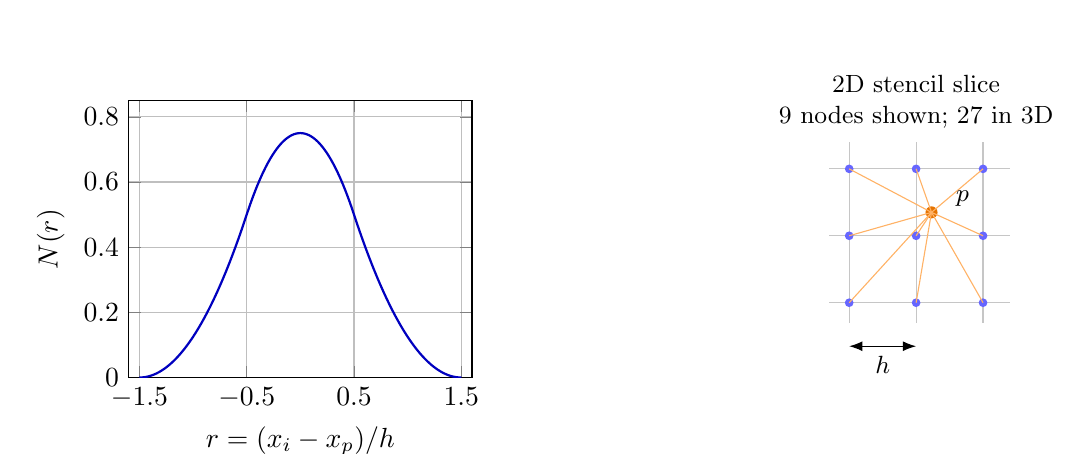
\begin{tikzpicture}
\begin{axis}[width=.49\textwidth,height=5.1cm,xlabel={$r=(x_i-x_p)/h$},
 ylabel={$N(r)$},xmin=-1.6,xmax=1.6,ymin=0,ymax=.85,
 xtick={-1.5,-.5,.5,1.5},grid=major,domain=-1.5:1.5,samples=151]
 \addplot[blue!75!black,thick] {abs(x)<0.5 ? 0.75-x*x : 0.5*(1.5-abs(x))^2};
\end{axis}
\begin{scope}[shift={(10,1.8)},scale=.85,>=Latex,font=\small]
 \draw[step=1,gray!45] (-1.3,-1.3) grid (1.4,1.4);
 \foreach \x in {-1,0,1}{\foreach \y in {-1,0,1}{\fill[blue!60] (\x,\y) circle (.065);}}
 \fill[orange!90!black] (.23,.35) circle (.09);
 \foreach \x in {-1,0,1}{\foreach \y in {-1,0,1}{\draw[orange!60,thin] (.23,.35)--(\x,\y);}}
 \node[anchor=west] at (.45,.55) {$p$};
 \draw[<->] (-1,-1.65)--node[below]{$h$}(0,-1.65);
 \node[align=center] at (0,2) {2D stencil slice\\9 nodes shown; 27 in 3D};
\end{scope}
\end{tikzpicture}
\caption{Analytical interpolation kernel and an illustrative stencil slice.
These are method diagrams, not simulation output. Exactly zero-weight stencil
entries must not create duplicate active grid nodes.}
\label{fig:kernel}
\end{figure}

\subsection{Particle-to-grid transfer and explicit stress force}
The implemented MLS-MPM transfer \cite{mlsmpm} combines affine momentum and an
explicit stress impulse:
\begin{align}
 m_i&=\sum_pw_{ip}m_p,\\
 \mathbf{p}_i^*&=\sum_pw_{ip}\left[m_p\mathbf{v}_p+
 \left(m_p\mathbf{C}_p-\Delta t\frac4{h^2}V_{0p}\boldsymbol\tau_p\right)
          \mathbf{d}_{ip}\right], \label{eq:p2g}\\
 \mathbf{v}_i^*&=\frac{\mathbf{p}_i^*}{m_i}+\Delta t\mathbf{g},\quad m_i>0.
\end{align}
In weak-form language the stress contribution is
$-\Delta t\sum_pV_{0p}\boldsymbol\tau_p\nabla w_{ip}$ with the MLS gradient
surrogate $\nabla w_{ip}\simeq(4/h^2)w_{ip}\mathbf{d}_{ip}$.
Dimensional check: $V_0\tau$ has units of energy; multiplying by
$\Delta t\,\mathbf{d}/h^2$ gives momentum.
Equation~\eqref{eq:moment-identities} cancels internal stress impulses in the
sum over nodes. That cancellation can fail in bookkeeping if an active node
is processed twice; the zero-deposit regression explicitly guards this case.

\subsection{Wall treatment, transfer back, and local update}
At a wall with inward unit normal $\mathbf{n}$, let
$v_n=\mathbf{v}^*\cdot\mathbf{n}$ and
$\mathbf{t}=\mathbf{v}^*-v_n\mathbf{n}$. Only $v_n<0$ is constrained:
\begin{equation}
 \mathbf{v}^{N}=\mathbf{t},\qquad
 \mathbf{v}^{+}=\mathbf{t}
 \max\left(0,1-\frac{\mu(-v_n)}{\|\mathbf{t}\|}\right), \label{eq:wall-projection}
\end{equation}
with the sticking/zero-tangent case handled explicitly. Axis-aligned wall
constraints are applied sequentially at corners. This is a nodal velocity
projection with Coulomb tangential reduction. It is \emph{not} an incompressible
pressure-Poisson solve and does not enforce a pointwise watertight surface.

After wall and optional pellet coupling updates,
\begin{align}
 \mathbf{v}_p^{n+1}&=\sum_iw_{ip}\mathbf{v}_i^+,\\
 \mathbf{C}_p^{n+1}&=\frac4{h^2}\sum_iw_{ip}\mathbf{v}_i^+
                           \mathbf{d}_{ip}^{T}, \label{eq:g2p}\\
 \mathbf{x}_p^{n+1}&=\mathbf{x}_p^n+\Delta t\,\mathbf{v}_p^{n+1}.
\end{align}
Paste uses the trial elastic tensor
$\mathbf{F}_e^{\rm tr}=(\mathbf{I}+\Delta t\mathbf{C}_p^{n+1})\mathbf{F}_e^n$;
liquid advances its scalar $J$ with $\operatorname{tr}\mathbf{C}_p^{n+1}$.
The constitutive operations are given in Section~\ref{sec:constitutive}.
A locally implicit plastic return does not make the global momentum step
implicit: the stress in \eqref{eq:p2g} is the stored stress from the preceding
accepted state.

\subsection{Adaptive integration and transactional state}
The research solver forms a heuristic upper bound
\begin{equation}
 \Delta t_{\rm stab}=\min\left\{
 \frac{\mathrm{CFL}\,h}{c+\max_p\|\mathbf{v}_p\|},\quad
 \frac{h^2}{4\nu},\quad 0.2\sqrt{m_r/k_n},\quad
 \frac{\mathrm{CFL}\,h}{\|\mathbf{v}_r\|}\right\}, \label{eq:mpm-step}
\end{equation}
where viscous and rigid terms apply only when present/nonzero. Here $c$ is the
material wave speed and $\nu$ the implementation's kinematic diffusivity.
A recovery factor can reduce the candidate step further. Endpoint clipping
then lands on the requested record/final time. Nonfinite state, constitutive
failure or excessive displacement rejects the trial; the solver restores
physical history and ledgers, halves the recovery scale and retries. A minimum
step failure is reported instead of silently changing the physics.

The checkpoint persists limiter/rejection history. A timestep-refinement case
is not accepted merely because one step happened to reach the requested cap:
\nolinkurl{limited_steps} counts accepted steps that were limited before endpoint
clipping. This distinguishes the tested temporal axis from an adaptive method
that actually reused the same smaller steps at every requested resolution.

\paragraph{Implementation mapping.}
\path{core/src/mpm/grid.rs}: \nolinkurl{GridLayout::stencil}, \nolinkurl{Stencil},
\nolinkurl{Grid::deposit}. \path{core/src/mpm/particles.rs}: \nolinkurl{ParticleSet}.
\path{core/src/mpm/solver.rs}: \nolinkurl{Simulation::particle_to_grid},
\nolinkurl{grid_update}, \nolinkurl{grid_to_particle}, \nolinkurl{try_step},
\nolinkurl{stability_limit} and \nolinkurl{advance_to}.
\path{core/tests/grid_transfer.rs} tests zero-weight bookkeeping and momentum.

\section{Single-pellet coupling and energy accounting}
\label{sec:coupling}
\subsection{Impulse exchange, not a porous-mixture closure}
For a research pellet, the signed distance is the minimum distance to its
multisphere union. A grid node inside that union is constrained only when its
relative normal velocity is approaching. With node position $\mathbf{x}_i$,
\begin{equation}
 \mathbf{u}_r(\mathbf{x}_i)=\mathbf{v}_r+
       \boldsymbol\omega_r\times(\mathbf{x}_i-\mathbf{x}_r),\qquad
 \mathbf{u}_{\rm rel}=\mathbf{v}_i-\mathbf{u}_r(\mathbf{x}_i).
\end{equation}
Apply \eqref{eq:wall-projection} to $\mathbf{u}_{\rm rel}$, then add back
$\mathbf{u}_r$. If $\Delta\mathbf{p}_i=m_i(\mathbf{v}_i'-\mathbf{v}_i)$ is
the grid impulse, the pellet receives
\begin{equation}
 \Delta\mathbf{P}_r=-\sum_i\Delta\mathbf{p}_i,\qquad
 \Delta\mathbf{L}_r=-\sum_i(\mathbf{x}_i-\mathbf{x}_r)\times\Delta\mathbf{p}_i.
 \label{eq:coupling-impulse}
\end{equation}
Linear and angular action-reaction balance is explicit at this grid/pellet
exchange. The body's start-of-step velocity is used for all constrained nodes,
then the summed impulse updates the body. It is not a simultaneous finite-mass
contact solve, and the two kinetic-energy changes need not cancel or sum to a
nonpositive number. Resolution-dependent leakage, work accuracy and multiple
research pellets remain acceptance gaps.

The separate research pellet uses world angular momentum and cylinder inertia;
wall contact is spring-dashpot/Coulomb contact rather than the grid projection.
The two rigid-body implementations share concepts, not identical state formats
or all contact-history details.

\subsection{Species and linear momentum residuals}
For household species $s\in\{\text{wood},\text{waste solids},\text{water}\}$,
\begin{equation}
 r_s=\sum_{c\in\{B,D,F,R,E\}}M_{s,c}
   -M_{s,0}-M_{s,\rm added}. \label{eq:species-residual}
\end{equation}
The compartments are bed, drawer, floor, removed and evaporated, summed over
boxes where appropriate. Reclassification of intact wood into fines is not a
new source. The native check bounds each residual by
$\max(\SI{1e-12}{kg},10^{-6}M_{s,\rm expected})$.
This tests bookkeeping, not spatial distribution or transport accuracy.

For the research continuum and optional pellet, let $\mathbf{P}$ be the sum of
particle translational and pellet linear momentum. The diagnostic is
\begin{equation}
 \mathbf{r}_P=\mathbf{P}(t)+\mathbf{P}_{\rm out}(t)-\mathbf{P}(0)
 -\mathbf{I}_g-\mathbf{I}_{\rm wall}-\mathbf{I}_{r,\rm wall}.
\end{equation}
The internal coupling impulse is not subtracted a second time. Current closed
fixtures reject nonzero outflow even when it balances this ledger. Consequently,
``mass conserved including escaped material'' cannot conceal a wall leak.

\subsection{Why a stationary wall's projection loss is not external work}
For one normal wall projection, record
\begin{equation}
 \Delta E_N=\tfrac12m_i(\|\mathbf{v}^{N}\|^2-\|\mathbf{v}^*\|^2)
          =-\tfrac12m_i v_n^2\leq0,\qquad
 \Delta D_F=\tfrac12m_i(\|\mathbf{t}\|^2-\|\mathbf{v}^{+}\|^2)\geq0.
 \label{eq:wall-energy}
\end{equation}
Thus $\Delta K_{\rm grid}=\Delta E_N-\Delta D_F$ exactly, up to roundoff.
A stationary wall has zero external boundary work, since its boundary velocity
is zero. $E_N$ mixes impact-like kinetic loss with numerical operator splitting;
calling it wall work is physically misleading.

For example, a resting node given gravity velocity $-g\Delta t$ and then
projected back to zero loses $m_i g^2\Delta t^2/2$ on the transient grid each
step. Over duration $T$, this is $m_i g^2T\Delta t/2$, which vanishes linearly
with timestep. It does not mean the stationary wall physically absorbed that
amount of gravitational work from an unmoving particle.

The recorded mechanical energy is
\begin{equation}
 E_{\rm mech}=\sum_p\left[\tfrac12m_p\|\mathbf{v}_p\|^2
       -m_p\mathbf{g}\cdot\mathbf{x}_p+V_{0p}\Psi_p\right]
       +K_r-m_r\mathbf{g}\cdot\mathbf{x}_r. \label{eq:mechanical-energy}
\end{equation}
Here $K_r$ includes rigid rotation, while the particle kinetic sum does
\emph{not} include APIC affine kinetic modes. The accumulated diagnostic sum is
\begin{align}
 L_E&=E_N-D_F+W_{r,\rm contact}
      +\Delta K_{\rm coupling,grid}+\Delta K_{\rm coupling,rigid}-D_P,\nonumber\\
 r_E&=E_{\rm mech}(t)-E_{\rm mech}(0)-L_E. \label{eq:energy-residual}
\end{align}
$D_P\geq0$ is the constitutive plastic-loss estimate.
$W_{r,\rm contact}$ is the start-of-step contact-force work estimate; it includes
recoverable penalty-spring effects and is not pure dissipation. The coupling
terms are measured kinetic changes, not an invented cancellation assumption.

\textbf{Equation~\eqref{eq:energy-residual} is not a closed physical first law.}
Missing terms include particle/grid transfer and affine energy, liquid viscous
loss, complete contact spring/rotation bookkeeping and any outflow energy.
Gravity discretization can also contribute a defect. A small $r_E$ alone could
reflect cancellation; a nonzero value cannot simply be called conservation
success. Future energy acceptance needs a consistently discretized balance,
not a renaming of the residual.

\paragraph{Implementation mapping.}
\path{core/src/mpm/rigid.rs}: \nolinkurl{Pellet::signed_distance},
\nolinkurl{couple_grid}, \nolinkurl{Pellet::apply_impulse}.
\path{core/src/mpm/solver.rs}: \nolinkurl{Ledger},
\nolinkurl{Ledger::ledgered_energy}, \nolinkurl{Simulation::energy_residual},
\nolinkurl{Simulation::momentum_residual}.
\path{core/src/research.rs}: \nolinkurl{check_closed_state} and restore validation.
The restored initial mechanical-energy baseline is checked against a rebuilt
initial state; missing histories are rejected rather than fabricated as zero.

\section{Verification observables and actual refinement evidence}
\label{sec:verification}
\subsection{What the fixture observables measure}
The particle spacing at initialization is $s_p=h/2$. The reported surface
proxies are
\begin{equation}
 H_h=\max_p z_p+s_p/2,\qquad
 B_{x,h}=\max_p x_p-\min_p x_p+s_p,\qquad S_h=H_0-H_h.
 \label{eq:surface-proxies}
\end{equation}
These estimate height, horizontal extent and slump using particle extrema plus
an \emph{initial} spacing correction. They are not reconstructed deformed
particle surfaces or a continuum free-surface mesh. They can therefore have
quadrature and surface-estimation error in addition to solver error.

The hydrostatic error metrics compare every particle, including those next to
the bottom boundary, to the phase-appropriate reference in
Section~\ref{sec:constitutive}:
\begin{equation}
 e_{\rm rms}=\left[\frac1{N_p}\sum_p
 \left(\frac{q_p-q_{\rm ref}(z_p)}{\rho_0gH_0}\right)^2\right]^{1/2},
 \qquad e_{\max}=\max_p\frac{|q_p-q_{\rm ref}(z_p)|}{\rho_0gH_0}.
\end{equation}
For liquid $q=p$ is pressure; for paste it is negative vertical Kirchhoff stress.
Removing bottom-row particles or smoothing per-particle liquid pressure would
change the acceptance question, not solve the observed accuracy problem.
The archived dataset below contains slump results only; it establishes no
hydrostatic-pressure convergence claim.

The code also reports a cylinder-slump sanity estimate \cite{pashias},
\begin{equation}
 Y=\frac{\tau_y}{\rho_0gH_0},\qquad
 \frac{S_{\rm cyl}}{H_0}=1-2Y[1-\ln(2Y)],\quad 0<Y<\tfrac12.
\end{equation}
It uses zero slump for $Y\geq1/2$ and $H_0$ for $Y\leq0$.
For $\tau_y=\SI{30}{Pa}$, $\rho_0=\SI{1000}{kg.m^{-3}}$,
$H_0=\SI{20}{mm}$ and $g=\SI{9.81}{m.s^{-2}}$, $Y\simeq0.152905$ and
$S_{\rm cyl}\simeq\SI{6.63737}{mm}$. The simulated block is a \emph{cube},
with finite elasticity, wall friction and time-dependent rheology. A mismatch
with this cylinder estimate is not by itself a validated error measure for
that different problem.

\subsection{Separate spatial and temporal experiments}
For observable $Q$ at three or more successively finer resolutions, the
implemented criterion computes
\begin{equation}
 \epsilon_k=\frac{|Q_k-Q_{k-1}|}{\max(|Q_k|,Q_{\rm scale})},\qquad
 \epsilon_{\rm final}<0.05. \label{eq:refinement}
\end{equation}
A finest value below $Q_{\rm scale}$ is \emph{uninformative}, not a pass. The
threshold is strict. Missing/nonfinite values, incomplete runs, changed fidelity,
wrong final times, adaptive limiting, rejected steps and budget overruns prevent
passing claims. The spatial axis holds the requested timestep fixed; the temporal
axis holds $h$ fixed and requires increasing actual step counts.

Three values can expose a failure to resolve an observable, but a small final
change does not prove asymptotic convergence. For equal refinement ratio $r$,
\begin{equation}
 p_{\rm obs}=\frac{\ln\left(|Q_0-Q_1|/|Q_1-Q_2|\right)}{\ln r}
\end{equation}
is merely a trend diagnostic without a verified leading-error expansion.
Neither Richardson extrapolation nor a formal discretization uncertainty bound
is claimed by this study.

The frozen run uses \path{examples/research_slump.yaml}, modified only by the
study axes in \path{examples/verification_slump.yaml}: a \SI{20}{mm} cube in a
\SI{60}{mm} domain, $\rho_0=\SI{1000}{kg.m^{-3}}$, $E=\SI{1000}{Pa}$,
$\nu_P=0.2$, $\tau_y=\SI{30}{Pa}$, $K_s=\SI{10}{Pa.s^{0.6}}$,
$n=0.6$, seed 7, final time \SI{0.5}{s}. All material values are synthetic.
The undeformed block mass is \SI{\BlockMassGrams}{g}, with continuum initial
potential energy $mgH_0/2=\SI{\BlockPotentialMillijoules}{mJ}$.
Non-hydrostatic fixtures add bounded position jitter of amplitude $0.1s_p$;
therefore the discrete initial potential energy differs slightly from this
integral. Spatial refinement also refines particle quadrature and jitter
amplitude; it is not a grid-only experiment with fixed material points.

\begin{table}[htbp]
\centering\small
\begin{tabular}{lrrrrrr}
\toprule
Axis & $h$ (mm) & $\Delta t$ (ms) & Points & Steps & Slump (mm) & Spread (mm) \\
\midrule
Spatial & 10 & 0.05 & 64 & 10000 & 3.9897 & 22.6655 \\
Spatial & 5 & 0.05 & 512 & 10000 & 4.3623 & 23.5512 \\
Spatial & 2.5 & 0.05 & 4096 & 10000 & 4.5165 & 25.9463 \\
Temporal & 5 & 0.4 & 512 & 1250 & 4.7376 & 25.0541 \\
Temporal & 5 & 0.2 & 512 & 2500 & 4.6077 & 24.6164 \\
Temporal & 5 & 0.1 & 512 & 5000 & 4.4875 & 24.1053 \\
\bottomrule
\end{tabular}

\caption{Actual compiled-kernel results at \SI{0.5}{s}, source revision
\nolinkurl{9a66a55}. Every case completed with zero limited and rejected steps.
Times and lengths here are requested caps/grid scales and measured final
surface proxies, respectively.}
\label{tab:cases}
\end{table}

\begin{figure}[p]
\centering
\begin{tikzpicture}
\begin{groupplot}[group style={group size=3 by 2,horizontal sep=1.5cm,vertical sep=2cm},
 width=.295\textwidth,height=.25\textheight,
 xmode=log,log basis x=2,x dir=reverse,grid=major,
 tick label style={font=\footnotesize},label style={font=\small},
 title style={font=\small},scaled ticks=false]
\nextgroupplot[title={Slump},xlabel={$h$ (mm)},ylabel={mm},xtick={10,5,2.5},
 xticklabels={10,5,2.5}]
\addplot+[blue!75!black,mark=*,thick] table[x=h_mm,y=slump_mm,col sep=comma]{generated/spatial.csv};
\nextgroupplot[title={Horizontal spread},xlabel={$h$ (mm)},ylabel={mm},xtick={10,5,2.5},
 xticklabels={10,5,2.5}]
\addplot+[blue!75!black,mark=*,thick] table[x=h_mm,y=spread_mm,col sep=comma]{generated/spatial.csv};
\nextgroupplot[title={Plastic-loss estimate},xlabel={$h$ (mm)},ylabel={$\mu$J},xtick={10,5,2.5},
 xticklabels={10,5,2.5}]
\addplot+[blue!75!black,mark=*,thick] table[x=h_mm,y=plastic_uj,col sep=comma]{generated/spatial.csv};
\nextgroupplot[xlabel={$\Delta t$ (ms)},ylabel={mm},xtick={.4,.2,.1},
 xticklabels={0.4,0.2,0.1}]
\addplot+[orange!85!black,mark=square*,thick] table[x=dt_ms,y=slump_mm,col sep=comma]{generated/temporal.csv};
\nextgroupplot[xlabel={$\Delta t$ (ms)},ylabel={mm},xtick={.4,.2,.1},
 xticklabels={0.4,0.2,0.1}]
\addplot+[orange!85!black,mark=square*,thick] table[x=dt_ms,y=spread_mm,col sep=comma]{generated/temporal.csv};
\nextgroupplot[xlabel={$\Delta t$ (ms)},ylabel={$\mu$J},xtick={.4,.2,.1},
 xticklabels={0.4,0.2,0.1}]
\addplot+[orange!85!black,mark=square*,thick] table[x=dt_ms,y=plastic_uj,col sep=comma]{generated/temporal.csv};
\end{groupplot}
\end{tikzpicture}
\caption{Frozen simulation evidence, \emph{not} illustrative curves. Top row:
spatial refinement at fixed $\Delta t=\SI{0.05}{ms}$. Bottom row: temporal
refinement at fixed $h=\SI{5}{mm}$. Each axis becomes finer to the right;
lines connect only the three observed values and are not fitted convergence
curves. Vertical axes are independent between panels. The study remains
unresolved because spread and plastic loss fail the specified final-two tests.}
\label{fig:refinement}
\end{figure}

\begin{table}[htbp]
\centering
\begin{tabular}{lrrr}
\toprule
Final-two change & Slump & Spread & Plastic loss \\
\midrule
Spatial & 3.41\% & 9.23\% & 31.39\% \\
Temporal & 2.68\% & 2.12\% & 10.25\% \\
\bottomrule
\end{tabular}

\caption{Final-two relative changes computed with \eqref{eq:refinement}.
Required: each listed value strictly below 5\%. Near-zero scales are
\SI{0.5}{mm} for lengths and \SI{1}{\micro J} for plastic loss.}
\label{tab:verdicts}
\end{table}

At $h=\SI{5}{mm}$ and $\Delta t=\SI{0.1}{ms}$, the recorded values include
\begin{align}
 E_N&=-\SI{109.379}{\micro J}, &D_F&=\SI{35.486}{\micro J},\\
 D_P&=\SI{173.886}{\micro J}, &r_E&=\SI{84.476}{\micro J}.
\end{align}
The nonzero diagnostic is retained. It is neither a pass of energy closure nor
an external-wall-work measurement. The six-case study took approximately
\SI{11.86}{s} on the producing arm64, 10-core, 16 GiB machine, measured through
report evaluation (not the final report write). This is a tiny-fixture timing,
not evidence for full-box or multi-day feasibility.

\paragraph{Implementation mapping and evidence identity.}
\path{core/src/mpm/fixtures.rs}: \nolinkurl{FixtureSpec::shape_observables},
\nolinkurl{slump_observables}, \nolinkurl{hydrostatic_observables}.
\path{python/litter_physics/verification.py}: \nolinkurl{plan_cases},
\nolinkurl{evaluate_observable}, \nolinkurl{evaluate_axis}, \nolinkurl{run_study}.
The verbatim archived report is \path{docs/formal/data/refinement-report.json};
its source commit, clean-tree flag, native/Python hashes, dependency versions,
hardware, all case values and unresolved verdicts are retained. The manuscript
build verifies the archive's SHA-256 before extracting any plot or table data.

\section{Calibration, reduced responses, and uncertainty}
\label{sec:calibration}
\subsection{What can currently be fitted}
The Python calibration module contains bounded empirical fits including
\begin{equation}
 U(t)=C[1-e^{-k_ut}],\qquad B(t)=1-e^{-k_bt},\qquad
 \tau(\dot\gamma)=\tau_y+K_s\dot\gamma^n.
\end{equation}
Tilt observations supply a friction prior based on $\tan\theta$; they do not
uniquely identify all multisphere sliding, rolling and shape parameters.
Visit observations fit stage statistics and can be held out for personalization
scoring. Synthetic observations remain explicitly synthetic; fit recovery from
synthetic data cannot identify a real cat or material.

There is an important model discrepancy: the fitted breakup fraction $B(t)$
is exponential, whereas the household runtime uses the accumulated,
whole-pellet threshold in \eqref{eq:damage}. Transferring $k_b$ between them does
not automatically calibrate the distribution of actual breakup times. A
simulator-based likelihood, an explicit heterogeneous threshold population, or
measured justification of the reduction is still needed. Likewise, fitting a
flow curve alone does not identify bulk elasticity, adhesion or porosity.

A prospective joint inverse problem can be written
\begin{equation}
 \widehat{\boldsymbol\theta}=\arg\min_{\boldsymbol\theta\in\Theta}
 \sum_j\frac{[\mathcal H_j(\mathcal S(\boldsymbol\theta))-y_j]^2}
                 {s_j^2}+\mathcal R(\boldsymbol\theta), \label{eq:inverse}
\end{equation}
where $\mathcal S$ is the simulator, $\mathcal H_j$ the measurement operator,
$y_j$ data, $s_j$ uncertainty/repeatability, and $\mathcal R$ a justified prior.
\textbf{Equation~\eqref{eq:inverse} is a proposed formulation, not an implemented
end-to-end inference engine.} Current functions fit the separate empirical
curves; unidentifiable parameter combinations must not be hidden by a low
training residual.

\subsection{Intended research-to-household response interface}
The implemented standalone response-table class provides bounded multilinear
interpolation on a full Cartesian grid. For a cell with lower/upper axis values
$x_j^-,x_j^+$, set $\lambda_j=(x_j-x_j^-)/(x_j^+-x_j^-)$:
\begin{equation}
 \widehat R(\mathbf{x})=\sum_{\mathbf b\in\{0,1\}^d}
 R_{\mathbf b}\prod_{j=1}^d
       \lambda_j^{b_j}(1-\lambda_j)^{1-b_j}. \label{eq:interpolation}
\end{equation}
Inside the cell the weights are nonnegative and sum to one. For example, a
hypothetical two-axis cell at $(\lambda_1,\lambda_2)=(1/4,1/2)$ has weights
$(3/8,1/8,3/8,1/8)$ under a compatible corner ordering. Interpolation is exact
for multilinear data, not for arbitrary nonlinear coupled material behavior.

The class validates grid completeness, units/physical bounds and evidence
provenance. It refuses absent/synthetic evidence and extrapolation by default;
explicit exploratory extrapolation is bounded to 10\% of each axis span and
still subject to response bounds. This mechanism does \emph{not} produce
validated evidence. No physical response tables are shipped, and neither native
mode currently consumes these tables. The dashed bridge in
Figure~\ref{fig:architecture} is intentionally not an implemented feedback loop.

A defensible future acceptance chain is: constitutive/balance tests; independent
space, timestep and domain-size studies; clean-surrogate measurements with
held-out errors no greater than 20\% or measured repeatability; then evidence-
qualified response reduction and measured household tests. Material variation,
parameter uncertainty, numerical error and behavior variability must be reported
separately. A confidence interval on a fitted parameter does not absorb unknown
model discrepancy.

\paragraph{Implementation mapping.}
\path{python/litter_physics/calibration.py}: \nolinkurl{fit_uptake},
\nolinkurl{fit_breakup}, \nolinkurl{fit_rheology}, \nolinkurl{friction_prior},
\nolinkurl{score_personalization}, \nolinkurl{apply_bundle}.
\path{python/litter_physics/response_tables.py}: \nolinkurl{ResponseTable},
\nolinkurl{Axis}, \nolinkurl{Evidence}, \nolinkurl{Evaluation}.


\section{Computational contract, reproducibility, and acceptance gaps}
\subsection{Execution and restart semantics}
Python validates requests and delegates bulk JSON calls to the PyO3 native
extension. Rust returns status, metrics, frames and full checkpoint state.
Python publishes immutable run segments containing JSON, Parquet and Rerun
artifacts, with configuration, code/build and dependency identity. Replay is
served on loopback; its browser URL explicitly names the recording source.
A rendered trajectory is an inspection tool, not a validation measurement.

Resuming requires matching frozen request/provenance and compatible native and
Python builds. Native restore validates physical/history/adaptive state as well
as geometry and baseline ledgers. A checkpoint lacking required history is
rejected instead of assigning unearned zero dissipation or limiter counts.
Atomic exclusive publication prevents competing writers from silently replacing
an existing run.

Research jobs have a one-hour local per-job target budget. Checks are cooperative
and include initialization/output budgeting, but do not preempt an expensive
operation or guarantee an exact wall-clock cutoff during finalization. An
incomplete run preserves a checkpoint and reports incompleteness. It must not
quietly switch to cheaper constitutive laws. Resource caps are guards, not
performance guarantees; a schema-valid request may still be infeasible.

\subsection{Scaling calculation, not an extrapolated benchmark}
For the \SI{20}{mm} cube with two points per cell per axis,
\begin{equation}
 N_p=\prod_{\alpha=1}^3\frac{L_\alpha}{h/2}
       =\left(\frac{2L}{h}\right)^3.
\end{equation}
This gives 64, 512 and 4096 points at $h=10,5,2.5$ mm. A P2G/G2P sweep touches
27 stencil nodes per point. Ignoring constants, occupied-grid work and output,
\begin{equation}
 \text{transfer work}\sim N_p\,\frac{T}{\Delta t};\qquad
 \begin{cases}
 O(h^{-4}),&\Delta t\propto h\text{ under an acoustic limit},\\
 O(h^{-5}),&\Delta t\propto h^2\text{ under a viscous limit}.
 \end{cases}
\end{equation}
Therefore halving $h$ can multiply this work by 16 or 32, not merely 8.
Neither scaling law is a measured runtime prediction: active sparsity, cache
behavior, return mapping, retries, sorting, contact and output all matter.
The present household scheduler does not establish adaptive multi-day idle
integration or actual-size runtime acceptance.

\subsection{Explicitly unresolved physics and numerical acceptance}
\begin{itemize}
 \item Hydrostatic bottom-boundary accuracy and liquid per-particle pressure
 noise remain unresolved. This document introduces no smoothing or weaker
 acceptance metric to make them disappear.
 \item Slump spatial spread and plastic-loss refinement fail the recorded
 threshold. Domain-size and combined space-time studies are still missing.
 \item The energy ledger is a mixed numerical diagnostic, not physical closure.
 Coupled work, leakage and contact/transfer energy require further analysis.
 \item Porous fines, capillary transport, absorption, wet fragmentation and
 adhesion are not research continuum phases. Research fines are explicitly
 unsupported; multiple research pellets are not implemented.
 \item Household paste stresses, resolved spreading/reaction, calibrated slot
 flux, measured settled packing, entrances/enclosures/pads and quantitative
 burial/exposure metrics remain incomplete.
 \item Per-cat motion/force identification, measured clean-surrogate validation,
 held-out household predictions and a validated response bridge are absent.
\end{itemize}
These gaps delimit what can be inferred from the formal equations. Conservation,
a successful compile, a smooth replay or a small synthetic fit residual cannot
replace the missing acceptance evidence.

\clearpage
\appendix
\section{Equation-to-code navigation}
Links below pin the scientific source baseline, so later implementation changes
do not silently alter the meaning of the derivations. More detailed symbol
mappings appear next to the corresponding sections.

\small
\begin{longtable}{>{\raggedright\arraybackslash}p{.29\linewidth}>{\raggedright\arraybackslash}p{.65\linewidth}}
\toprule
Formal component & Source and role\\
\midrule\endhead
State map \eqref{eq:state-map}, inputs &
\source{python/litter_physics/models.py}: requests and domain validation.
\source{core/src/lib.rs}: native mode dispatch.\\[.6em]
Rigid geometry and contacts, \eqref{eq:pellet-inertia}--\eqref{eq:dem-step} &
\source{core/src/dem.rs}: multisphere geometry, forces, history, integration and slots.\\[.6em]
Uptake/damage/swelling, \eqref{eq:uptake}--\eqref{eq:swelling} &
\source{core/src/household.rs}: stateful boxes, events and moisture histories.\\[.6em]
Reduced transport, \eqref{eq:drainage} &
\source{core/src/household/field.rs}: free water, fines, occupancy and drawer flux.\\[.6em]
Paste and liquid constitutive laws &
\source{core/src/mpm/constitutive.rs}: material conversion, local return and EOS.\\[.6em]
Stencil and transfers, \eqref{eq:weights}--\eqref{eq:g2p} &
\source{core/src/mpm/grid.rs}, \source{core/src/mpm/particles.rs},
\source{core/src/mpm/solver.rs}: grid support, particle history and stepping.\\[.6em]
Rigid impulse exchange, \eqref{eq:coupling-impulse} &
\source{core/src/mpm/rigid.rs}: research pellet, wall contact and grid coupling.\\[.6em]
Research residuals, \eqref{eq:wall-energy}--\eqref{eq:energy-residual} &
\source{core/src/mpm/solver.rs}: signed energy channels and state validation.
\source{core/src/research.rs}: closed-wire-fixture checks and checkpoint restore.\\[.6em]
Fixtures and observables, \eqref{eq:surface-proxies} &
\source{core/src/mpm/fixtures.rs}: initialization, surface proxies and diagnostic reference fields.\\[.6em]
Refinement criterion, \eqref{eq:refinement} &
\source{python/litter_physics/verification.py}: case plans, fail-closed evidence and verdicts.\\[.6em]
Behavior and empirical calibration &
\source{python/litter_physics/behavior.py},
\source{python/litter_physics/calibration.py}: visit distributions, fits and evidence labels.\\[.6em]
Response interpolation, \eqref{eq:interpolation} &
\source{python/litter_physics/response_tables.py}: standalone evidence-bounded interpolation,
not native dynamics.\\[.6em]
Run artifacts and replay &
\source{python/litter_physics/runner.py},
\source{python/litter_physics/artifacts.py},
\source{python/litter_physics/provenance.py},
\source{python/litter_physics/viewer.py}: orchestration and inspection.\\
\bottomrule
\end{longtable}
\normalsize

\clearpage
\section{Rebuilding the document and reproducing the experiment}
From the repository root, with the locked Python environment and Tectonic
installed:
\begin{verbatim}
make manuscript
uv run python docs/formal/build.py --check
uv run litter-physics verify examples/verification_slump.yaml \
    --out outputs/reproduce-formal-slump
\end{verbatim}
The build checks the archived report, generates deterministic CSV/LaTeX data,
and compiles this PDF. Method diagrams are vector TikZ drawings; the kernel
plot is analytic; Figure~\ref{fig:refinement} uses the archived native results.
No new physics run is hidden inside document compilation. The baseline study's
expected verification exit status is 1 (complete but unresolved), not 0.
Fresh run directories must be empty. Exact wall times and PDF bytes need not
match across platforms or tool versions; numerical data and provenance remain
inspectable.

The report's SHA-256 is
\begin{center}\small\path{aa6030d7ea1af0919343d3c4732855bce3eecc3c69310a7babc116dc0015bce8}.\end{center}
\path{docs/formal/README.md} documents compiler requirements, generated artifacts,
checks and the intentional historical source pin.

\begin{thebibliography}{9}
\bibitem{cundall} P. A. Cundall and O. D. L. Strack.
\emph{A discrete numerical model for granular assemblies}.
G\'eotechnique, 1979. \url{https://doi.org/10.1680/geot.1979.29.1.47}.
\bibitem{apic} C. Jiang, C. Schroeder, A. Selle, J. Teran and A. Stomakhin.
\emph{The affine particle-in-cell method}.
ACM Transactions on Graphics, 2015. \url{https://doi.org/10.1145/2766996}.
\bibitem{mlsmpm} Y. Hu, Y. Fang, Z. Ge, Z. Qu, Y. Zhu, A. Pradhana and C. Jiang.
\emph{A moving least squares material point method with displacement
discontinuity and two-way rigid body coupling}.
ACM Transactions on Graphics, 2018. \url{https://doi.org/10.1145/3197517.3201293}.
\bibitem{foam} Y. Yue, B. Smith, C. Batty, C. Zheng and E. Grinspun.
\emph{Continuum Foam}. ACM Transactions on Graphics, 2015.
\url{https://doi.org/10.1145/2751541}.
\bibitem{pashias} N. Pashias, D. V. Boger, J. Summers and D. J. Glenister.
\emph{A fifty cent rheometer for yield stress measurement}.
Journal of Rheology, 1996. \url{https://doi.org/10.1122/1.550780}.
\end{thebibliography}
\end{document}
